\documentclass[10pt]{beamer}

\usepackage[utf8]{inputenc}
\usepackage{pgfpages}
\usepackage{dirtree}
\setbeamertemplate{note page}[plain]
\AtEndNote{\vfill \begin{center} mm:hh \end{center}}
\newcommand{\notedir}[1] {
  \note{\dirtree{#1}}}
\def \ion {$^{\circ}$ }
\usepackage{tcolorbox}
\usepackage{tikz}
\usepackage{tikz-3dplot}
\usetikzlibrary{intersections,calc,angles,quotes}
\usepackage{amsmath}
\usepackage{graphicx}
\usepackage{cases}
\def \heart {\textcolor{blue}{$\heartsuit$} }
\def \C {\mathcal{C}}
\def \orthog {\underline{\perp}}
\def\arcos{\operatorname{arcos}}

\tcbset{%
	basic/.style={colframe=black,
		      colback=white,
		      top= 0mm,
		      bottom = 2mm,
		      boxsep=0mm
		      }
}
\tikzset{
    invisible/.style={opacity=0},
    visible on/.style={alt={#1{}{invisible}}},
    alt/.code args={<#1>#2#3}{%
      \alt<#1>{\pgfkeysalso{#2}}{\pgfkeysalso{#3}} % \pgfkeysalso doesn't change the path
    },
  }

  \def\enonce{ \frametitle{Q1 Juillet 2001.}
	  %\renewcommand{\theenumi}{\alph{enumi})}
	   Soient $ABC$ un triangle et $\C$ son cercle circonscrit. \\
	  On note $A'$ le point d’intersection de $\C$ avec la médiatrice du segment $[B, C]$ qui
	  est tel que $A$ et $A'$ soient situés de part et d’autre de la droite $BC$.
	  Les points $B'$ et $C'$ sont définis de façon analogue : $B'$ sur $\C$ et la médiatrice du
	  segment $[A, C]$, $C'$ sur $\C$ et la médiatrice du segment $[B, C]$, $B$ et $B'$ de part et
	  d’autre de $AC$, $C$ et $C'$ de part et d’autre de $AB$. \\
	  Prouver que les droites $AA'$ , $BB'$ et $CC'$ sont concourantes.
  }
  \def\hypotheses{  \underline{Hypothèses} 
				    \begin{enumerate}
				    \item $A'A_1$ médiatrice de $BC$, \\
					  $B'B_1$ médiatrice de $AC$, \\
					  $C'C_1$ médiatrice de $AB$. \\
				    \item $\C$ cercle circonscrit à $ABC$.
				    \end{enumerate}
  }
  \def\these{  \underline{Thèse} \\
		      \smallskip
		      $AA'$ , $BB'$ et $CC'$ concourantes.
    }
    
\begin{document}  
    \beamertemplatenavigationsymbolsempty
    \setlength{\abovedisplayskip}{0pt}
    \setlength{\belowdisplayskip}{0pt}
    \frame{
	  \enonce
	 
	  \vfill
	  
	  \pause
	  % hypothèses et thèse
	  \begin{tcolorbox}[basic] 
	      \begin{columns}[t]
		 
		 \column{.5\textwidth}\centering
		      
		      \hypotheses
		      {\small $A_1,B_1,C_1$ pied des médiatrices.}
		  
		  \column{.5\textwidth}\centering
		      
		   \these
		
	      \end{columns}
	  \end{tcolorbox}
	  \notedir{%
	.1 Énoncé.
	.2 Hypothèses (non visibles sur le dessin)..
	.2 Thèse..
	.2 Grand dessin.. 
	}
    }

    \frame{ 
	  % résolution ex1
	  \begin{columns}[t]
		\column{.52\textwidth}\centering 
		

			\underline{Dessin}\\
			
				  \begin{figure}[h]
				  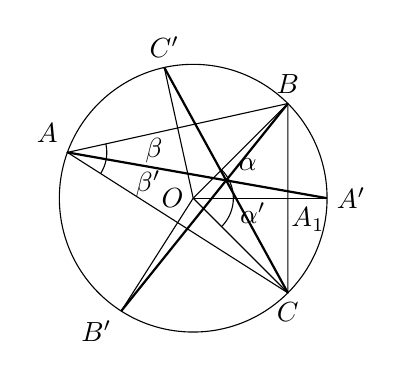
\begin{tikzpicture}[scale=0.85]
			          %projection ($(X)!(B')!(B)$)
			          %nommer chemin 'name path
			          %intersection \path [name intersections={of=d and gb,by=G}];
			          
			          %\draw[help lines] (-3,-3) grid (3,3);
			          %Cercle et triangle
			          \coordinate[](O) at (0,0);
			          \coordinate[label=above:$B$](B) at (45:2);
			          \coordinate[label=below:$C$](C) at (-45:2);
			          \coordinate[label=above left:$A$](A) at (160:2);			          
			          \draw[name path=cercle] (O) circle (2);
			          \draw (A) -- (B) -- (C) -- cycle;
			          
			          %A',A_1,B',B_1,C',C_1
				  \coordinate (A') at (0:2);
			          \coordinate (A_1) at (1.414,0);
			          \coordinate (C_1) at ($0.5*(A)+0.5*(B)$);
			          \path[name path=OC_1] (O) -- ($2*(C_1)$);
			          \path [name intersections={of=OC_1 and cercle,by=C'}];
			          \coordinate (B_1) at ($0.5*(A)+0.5*(C)$);
			          \path[name path=OB_1] (O) -- ($5*(B_1)$);
			          \path [name intersections={of=OB_1 and cercle,by=B'}];
			          
			          \draw[visible on=<{1,2}>] (O) node[left] {$O$} -- (A');
			          \draw[visible on=<{1,2}>] (A') node [right]{$A'$};
			          \draw[visible on=<{1}>] (O) -- (B');
			          \draw[visible on=<{1}>] (B') node [below left]{$B'$};
			          \draw[visible on=<{1}>] (O) -- (C');	
			          \draw[visible on=<{1}>] (C') node [above]{$C'$};
			          \draw[thick,visible on=<{1,2}>] (A) -- (A');
			          \draw[thick,visible on=<{1}>] (B) -- (B');
			          \draw[thick,visible on=<{1}>] (C) -- (C');			         
				  
			       
			          \draw[visible on=<2>] (O) -- (A_1) node[below right,xshift=-0.8mm] {$A_1$};
			          \draw[visible on=<2>] (O) -- (B);
			          \draw[visible on=<2>] (O) -- (C);
			          %angles
			          \draw[visible on=<2>] (0.6,0) arc[radius = 6mm, start angle= 0, end angle= 45] node [above right,pos=0.6]{$\alpha$};
				  \draw[visible on=<2>] (0.6,0) arc[radius = 6mm, start angle= 0, end angle= -45] node [right,pos=0.5]{$\alpha '$};
				  \pic [draw, visible on=<2>,"$\beta '$", angle eccentricity=2.2] {angle = C--A--A'};
				  \pic [draw, visible on=<2>,"$\beta$", angle eccentricity=2.2] {angle = A'--A--B};
				  \end{tikzpicture}
				  \end{figure}
			
				  \begin{tcolorbox}[basic] 
				      
				    \smallskip
				  \hypotheses
							      
				    \these
				    \end{tcolorbox}
		
		
		\column{.59\textwidth}\centering
		
		\underline{Résolution}\\ \flushleft

                
		\onslide<+->	\heart Les bissectrices d'un $\Delta$ sont concourantes.\\
                $\rightarrow$ Montrer que $AA',BB',CC'$ sont bissectrices de $\Delta ABC$.\\[1em]
                \heart  Les médiatrices d'un triangle se coupent au centre du cercle circonscrit. \\$\rightarrow O$ est le centre de $\mathcal{C}$. \\[1em]
		\onslide<+-> \heart Un angle inscrit mesure la moitié de l'angle au centre interceptant le même arc.
                 $$  \beta  = \frac{\alpha }{2} \quad \beta ' = \frac{\alpha '}{2}$$\smallskip
                
                 Or  $\Delta OBA_1,\Delta OA_1C$ isométriques car :
$\begin{cases} [OA_1] \text{ en commun}, \\ |BA_1| = |A_1C|, (\textcolor{blue}{1.}) \\ \widehat{OA_1B}=\widehat{OA_1C}=90^\circ.  (\textcolor{blue}{1.})\end{cases}\rightarrow \alpha = \alpha '$
                 \smallskip

           	
			    $\rightarrow \beta=\beta '\rightarrow AA'$ bissectrice de $ABC$ de $A$. 

   
	   \end{columns}
    \notedir{%
	   .1 Prouver thèse.
	   .2 $AA',BB',CC'$ concourantes.
	   .3 Élément de théorie.
	   .4 Les bissectrices d'un $\Delta$ sont concourantes (Les 3 droites ressemblent à bissectrices)..
	   .3 Résolution..
           .4 $O$ centre de $\mathcal{C}$ car médiatrices $\nmid$ au centre de $\mathcal{C}$..
	   .4 $AA'$ bissectrice issue de $A$ car $\beta = \beta '$ vu que.
            .5 L'angle au centre vaut double de celui inscrit et.
	   .6 $\alpha = \alpha '$ car $\Delta OA_1C, \Delta OA_1B$ isométriques (2 côtés et un angle égaux)..
	   }
         }
             \frame{ 
	  % résolution ex1
	  \begin{columns}[t]
		\column{.52\textwidth}\centering 
		

			\underline{Dessin}\\
			
				  \begin{figure}[h]
				  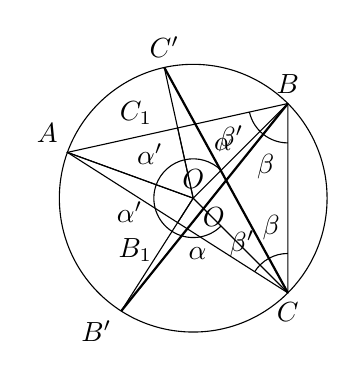
\begin{tikzpicture}[scale=0.85]
			          %projection ($(X)!(B')!(B)$)
			          %nommer chemin 'name path
			          %intersection \path [name intersections={of=d and gb,by=G}];
			          
			          %\draw[help lines] (-3,-3) grid (3,3);
			          %Cercle et triangle
			          \coordinate[](O) at (0,0);
			          \coordinate[label=above:$B$](B) at (45:2);
			          \coordinate[label=below:$C$](C) at (-45:2);
			          \coordinate[label=above left:$A$](A) at (160:2);			          
			          \draw[name path=cercle] (O) circle (2);
			          \draw (A) -- (B) -- (C) -- cycle;
			          
			          %A',A_1,B',B_1,C',C_1
				  \coordinate (A') at (0:2);
			          \coordinate (A_1) at (1.414,0);
			          \coordinate (C_1) at ($0.5*(A)+0.5*(B)$);
			          \path[name path=OC_1] (O) -- ($2*(C_1)$);
			          \path [name intersections={of=OC_1 and cercle,by=C'}];
			          \coordinate (B_1) at ($0.5*(A)+0.5*(C)$);
			          \path[name path=OB_1] (O) -- ($5*(B_1)$);
			          \path [name intersections={of=OB_1 and cercle,by=B'}];
			          			          \draw[visible on=<{1}>] (O) -- (B');
			          \draw[visible on=<{1}>] (B') node [below left]{$B'$};
			          \draw[visible on=<{2}>] (O) -- (C');	
			          \draw[visible on=<{2}>] (C') node [above]{$C'$};
			          \draw[thick,visible on=<{1}>] (B) -- (B');
			          \draw[thick,visible on=<{2}>] (C) -- (C');			         
				 
			          
			          \draw[visible on=<1>] (O) -- (B_1) node[ below left,xshift=-2mm,yshift=-0.8mm] {$B_1$};
			          \draw[visible on=<1>] (O) node[above] {$O$} -- (A);
			          \draw[visible on=<1>] (O) -- (C);
			          %angles
			          \pic [draw, visible on=<1>,left,"$\alpha '$", angle eccentricity=1.1] {angle = A--O--B'};
				  \pic [draw, visible on=<1>,below,"$\alpha$", angle eccentricity=1] {angle = B'--O--C};
				  \pic [draw, visible on=<1>,"$\beta '$", angle eccentricity=1.7] {angle = A--B--B'};
				  \pic [draw, visible on=<1>,"$\beta$", angle eccentricity=1.7] {angle = B'--B--C};
				  
				  \draw[visible on=<2>] (O) -- (C_1) node[ above left,xshift=-2mm,yshift=-0.8mm] {$C_1$};
			          \draw[visible on=<2>] (O) node[below right] {$O$} -- (A);
			          \draw[visible on=<2>] (O) -- (B);
			          %angles
			          \pic [draw, visible on=<2>,above left,"$\alpha '$", angle eccentricity=0.8] {angle = C'--O--A};
				  \pic [draw, visible on=<2>,above right,"$\alpha$", angle eccentricity=1] {angle = B--O--C'};
				  \pic [draw, visible on=<2>,"$\beta '$", angle eccentricity=1.7] {angle = C'--C--A};
				  \pic [draw, visible on=<2>,"$\beta$", angle eccentricity=1.7] {angle = B--C--C'};
				  \end{tikzpicture}
				  \end{figure}
			
				  \begin{tcolorbox}[basic] 
				      
				    \smallskip
				  \hypotheses
							      
				    \these
				    \end{tcolorbox}
		
		
		\column{.59\textwidth}\centering
		
		\underline{Résolution}\\ \flushleft

		\onslide<+-> De la même façon : \\ \smallskip
		$BB'$ bissectrice de $ABC$ issue de $B$. \\ \smallskip
		\onslide<+->$CC'$ bissectrice de $ABC$ issue de $C$. \\ \smallskip
                $\rightarrow AA', BB', CC'$ bissectrices de $\Delta ABC$ donc elles sont concourantes.
	 \hfill $\qed$
		%\centering\noindent\rule{2cm}{0.4pt}
	        %\hfill $\qed$

   
	   \end{columns}
    \notedir{%
	   .1 Prouver thèse.
	   .2 $AA',BB',CC'$ concourantes.
	   .3 Élément de théorie.
	   .4 Les bissectrices d'un $\Delta$ sont concourantes (Les 3 droites ressemblent à bissectrices)..
	   .3 Résolution..
           .4 $O$ centre de $\mathcal{C}$ car médiatrices $\nmid$ au centre de $\mathcal{C}$..
	   .4 $AA'$ bissectrice issue de $A$ car $\beta = \beta '$ vu que.
            .5 L'angle au centre vaut double de celui inscrit et.
	   .6 $\alpha = \alpha '$ car $\Delta OA_1C, \Delta OA_1B$ isométriques (2 côtés et un angle égaux)..
	   .4 De la même façon, $BB',CC'$ sont bissectrices..
	   .4 Les bissectrices d'un $\Delta$ sont concourantes..
	   }
         }


	             \frame{ 
	  \enonce

	  \vfill\center
	  \underline{Résumé}\\ \flushleft
          \begin{itemize}
          \item Médiatrice d'un segment = droite $\perp$ au segment passant par son milieu.
            \item Montrer que 3 droites sont concourantes = est-ce des droites particulières d'un $\Delta$ ?
	  \item  Les bissectrices d'un $\Delta$ sont concourantes.
          \item  Les médiatrices d'un triangle se coupent au centre du cercle circonscrit.
            \item Un angle inscrit mesure la moitié de l'angle au centre interceptant le même arc.
          \end{itemize}
    }
	
  
\end{document}

%%% Local Variables:
%%% mode: latex
%%% TeX-master: t
%%% End:
